\chapter{Introduction}
\label{cha:introduction}

Human languages obey many regularities which have been studied and formalized into laws.
One of the most well known such laws is Zipf's law, which states that
\begin{equation}
  \label{eq:zipf_law}
  p(i) \sim i^{-\alpha}
\end{equation}
where $i$ is a word's rank.
Generally, $\alpha \approx 1$ \cite{Zipf1949a}.
This is the case not only for English but for every tested human language \cite{Mehri2017}.
Figure \ref{fig:zipf_languages_wiki} shows this relationship for the first 10 million words of Wikipedia dumps in 30 different languages.
This relationship also holds for artifical languages like Esperanto.
There have been many efforts to understand why this and other empiric laws occur consistently in human language.

\begin{figure}
  \centering
  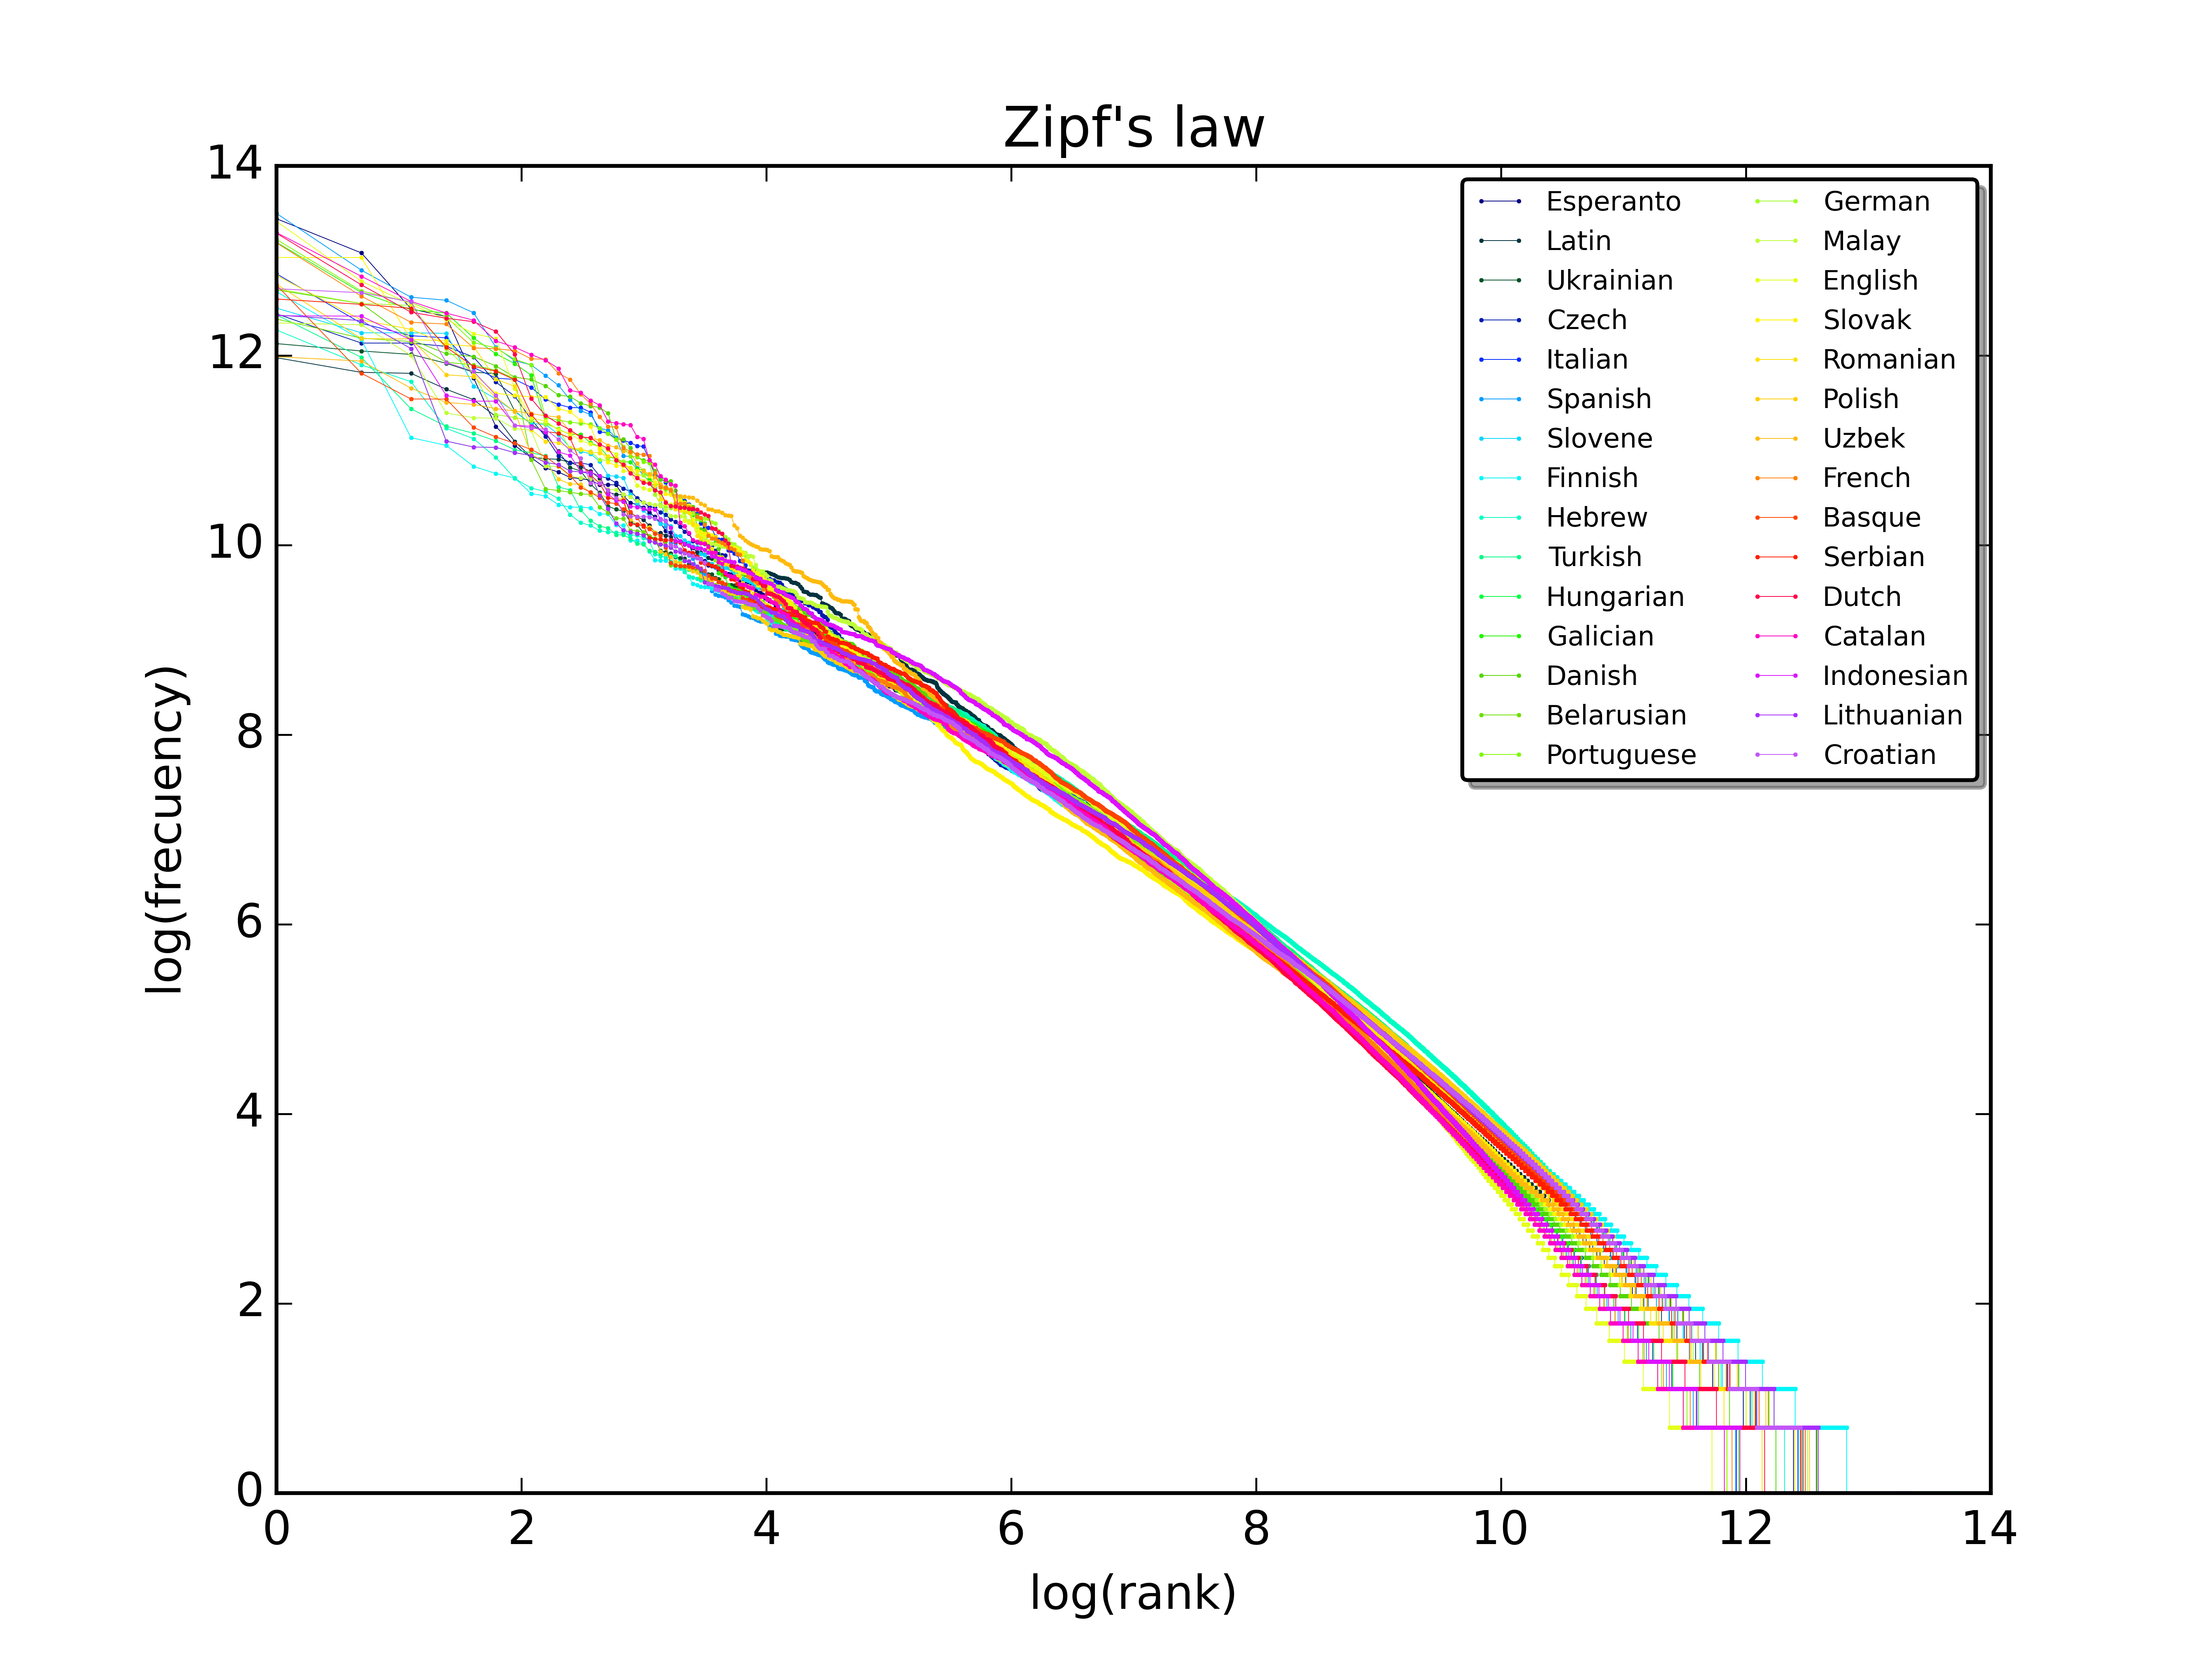
\includegraphics[width=\textwidth]{zipf_languages_wiki}
  \caption{
    The relationship of the logarithm of a word's frequency versus its rank for 30 human languages including Esperanto, an artifical language.
    Data from 30 Wikipedia dumps from October 2015.\\
    (Sergio Jimenez/Wikimedia, CC BY-SA 4.0 \cite{Jimenez2015a})}
  \label{fig:zipf_languages_wiki}
\end{figure}

This thesis focuses on a family of models \cite{Ferrer2007a} introduced initially to shed light into the origins of Zipf's law \cite{Ferrer2005a} \cite{Ferrer2003a}.
The focus of this thesis are two models from this family, which were generalized with the addition of a new parameter $\phi$. \cite{Ferrer2018a}
They are referred to as the ``\firstmodel{}'' and the ``\secondmodel{}'' throughout.
The key difference between these two models is whether they consider meanings to follow a probability distribution \emph{internal} or \emph{external} to the model.

It has been argued \cite{Ferrer2003a} \cite{Zipf1949a} that human language is result of attempting to minimize the effort of both the speaker and the hearer. Something that Zipf referred to as the \emph{principle of least effort}. These models follow this principle and are based on the minimization of a cost function, which is calculated in terms of information theoretic measures.

The motivation for this thesis is that these models could describe other language laws.
Zipf's law for word frequencies is quite well known but there are other patterns in human language.
One such pattern is the meaning-frequency law, also first reported by Zipf in his book. \cite{Zipf1949a}
Another is the relationship between the age of a word and its frequency, also studied by Zipf. \cite{Zipf1949a}
The consistent appearance of this law in 

In order to study these patterns in the model, a \CC{} program is implemented as part of this thesis.
This program is flexible and powerful enough to replicate previous results \cite{Ferrer2003a} \cite{Ferrer2005a} and also capable of generating results for newer versions of these models.
This program is one of the major contributions of this thesis.
It is released under an open source license with the hope that it can help others study these models and similar ones.

The rest of this chapter is divided as follows.
Section \ref{sec:introduction_background} revises the state of the art.
Previous articles about this family of models along with their responses and critiques, until the more current models are reached.
Section \ref{sec:introduction_general-goals} outlines the set of goals of this thesis without entering into detail about the models.
Section \ref{sec:introduction_model} introduces the family of models and the two models that are studied in detail.
Having introduced the model, section \ref{sec:introduction_goals} goes into more detail about the objectives of the thesis and section \ref{sec:introduction_hypothesis} covers the hypothesis.
Section \ref{sec:introduction_challenges} explains the main challenges that from this work.
Finally, Section \ref{sec:introduction_outline} outlines the rest of the thesis.

\section{Background}
\label{sec:introduction_background}

This section covers the ``state of the art'' or background of the thesis.
Section \ref{sec:introduction_background_linguistic-laws} explains some of the linguistic laws that have been found in more detail.
Section \ref{sec:introduction_background_similar} explores similar approximations to general problems and other models that have been proposed to explain Zipf's law, comparing them to these models.

\subsection{Linguistic laws}
\label{sec:introduction_background_linguistic-laws}

Here some space is dedicated to describe the linguistic laws that are studied in the model in more detail.

\subsubsection{Zipf's word-frequency law}

This law is well known as Zipf's law.
This thesis opens with its formulation in Equation \eqref{eq:zipf_law} due to its importance.
A word's frequency is inversely proportional to its rank when ordered by frequency.
The negative exponent $\alpha$ is typically around 1. \cite{Zipf1949a}

This is one of the most well known laws in quantitative linguistics and previous models were already seen to follow it \cite{Ferrer2003a} \cite{Ferrer2005a}.

\subsubsection{Zipf's meaning-frequency and meaning distribution laws}

Zipf's meaning-frequency law is less well known.
The law states the dependency between the number of meanings of a word $\mu$ and its frequency $f$, \cite{Zipf1949a}
\begin{equation*}
  \mu \propto f^\delta.
\end{equation*}
Zipf derived the meaning-frequency law from his famous law of word-frequency, Equation \eqref{eq:zipf_law} and from his law of meaning distribution,
\begin{equation*}
  \mu \propto i^{-\gamma}
\end{equation*}
where $i$ is the rank of the word and $\gamma \approx 1/2$

As with the constant $\alpha$, $\delta$ and $\gamma$ can be estimated using a regression method from data.

Zipf argued, and it has been proven \cite{Ferrer2016a} that
\begin{equation}
  \label{eq:relation-exponents}
  \delta = \frac{\gamma}{\alpha}.
\end{equation}

\subsubsection{Zipf's Age-frequency law}

Zipf argued in his book \cite{Zipf1949a} that older words (words that have existed in a language for a longer amount of time) would be more frequent.
This was tested empirically, as seen in Figure \ref{fig:zipf_word_ages}.

\begin{figure}
  \centering
  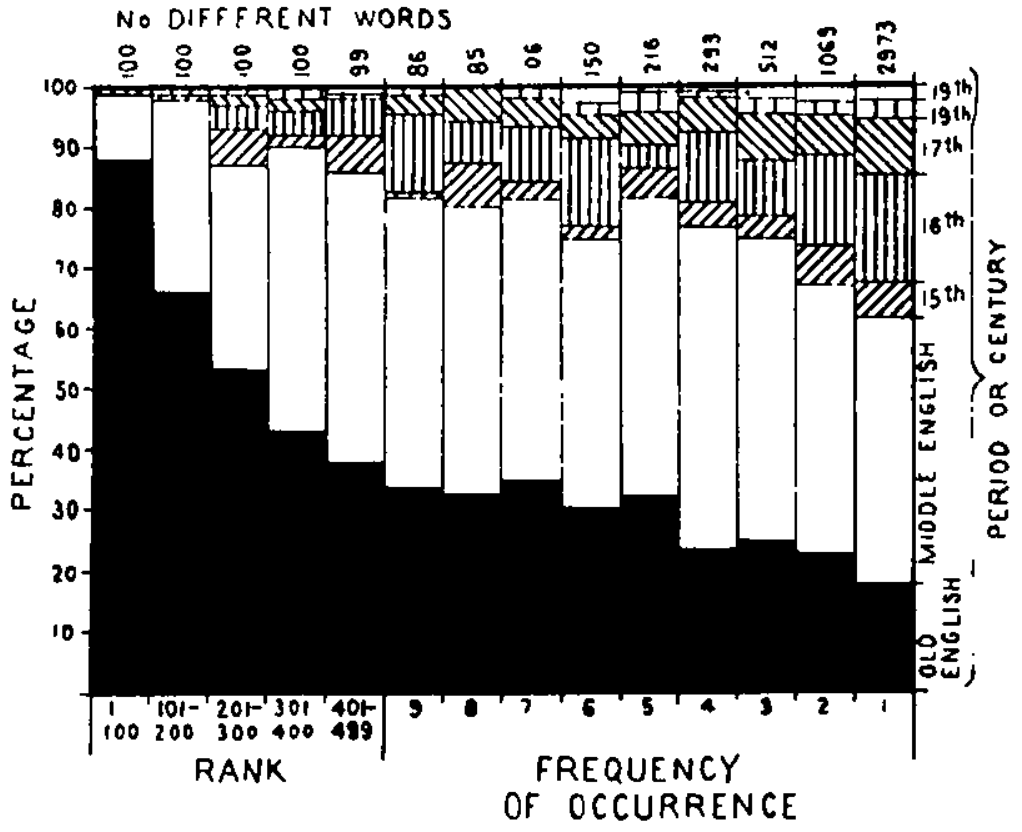
\includegraphics[width=\textwidth]{zipf_word_ages}
  \caption{
    Age of a word as a function of its frequency.
    The right side of the $y$ axis indicates the historical period or century when a word was introduced and the left side the percentage of words.
    Each of the colors and patterns of the columns in the graph correspond with a time period.
    As indicated in the $x$ axis, the first five columns refer to the most common words by rank, while the next columns refer to the words with the specified frequency of occurrence.
  }
  \label{fig:zipf_word_ages}
\end{figure}

\subsection{Similar research}
\label{sec:introduction_background_similar}

This section goes over other problems that have been solved similarly and other models that have attempted to explain Zipf's law.
A summary table between these alternative models and the models presented in this thesis is also shown.

\subsubsection{Similar approximations to general problems}

There has been research which can be related to the work done in this thesis.

Terry Regier argued \cite{Regier2007a} that color naming in human language corresponded with optimal partitions of the color space.
This is similar to the models presented here which, inspired by Zipf's \emph{principle of least effort}, consider language to be the result of optimizing speaker and hearer effort.
Regier's research showed that, indeed, color naming in many human languages was closely related to the optimal partitions of the color space.
The idea of language being ``optimal'' is not new.

In shortest path calculation algorithms, when a change takes place it is common to adjust the result based on the change instead of recalculating the entire process.
These changes offer speed ups of several orders of magnitude. \cite{Buriol2003a}
This is similar to the static vs dynamic approach (Section \ref{sec:introduction_model_dynamic-static}).
In this case, the dynamic algorithm offers a significant speedup that justifies issues such as the increase in mathematical complexity.

\subsubsection{Other models that explain Zipf's Law}

One of the most common explanations for Zipf's law is the random typing model.\cite{Miller1963a}
As a short summary, this model states that if characters are typed in sequence with a random chance of typing in a word separator then Zipf's law is reproduced.

While it is true that the Miller's random typing shows behavior similar to Zipf's law, it is also a shallow explanation that misses many important details.
To name a few issues, Miller's model assumes that words are independent from each other.
However, in human language, words are very much dependent on each other.
Random typing is often offered as a null hypothesis to the theory that Zipf's law comes from the \emph{principle of least effort}.
However, it has been shown \cite{Ferrer2020a} that random typing is an optimal coding process, which would make it not suitable as a null hypothesis either.

The random typing model would also not be able to explain other linguistic laws, such as the relationship between word age and frequency or the meaning distribution law, as it does not take into account the meanings nor the ages of words.
It could also not make more complex predictions, such as the vocabulary learning biases observed in children.

Another model which is used to explain the occurrences of power laws in nature is Simon's model.\cite{Simon1955}
This model argues that these power laws appear as a result of the way the system is formed.
In the case of language, constant addition of new words and addition of new instances of already existing words at a rate proportional to the number of instances of a word.

This model is not as widely known as the random typing model.
However, it is also not as powerful as the models presented in this thesis.
Like the random typing model, Simon's model cannot explain the meaning distribution law as it does not take meaning into account.
It also lacks the complexity to make predictions such as the vocabulary learning biases of children.
However, it could perhaps explain or at least try to predict the age frequency law, as the ages of words could be tracked.

Table \ref{tab:comparison_models} shows a comparison between the two models seen here (random typing and Simon's model) and the two models that this thesis presents.
The two models are further fleshed out in following sections.

\begin{table}
  \centering
  \begin{tabular}{p{2.5cm}p{1.5cm}p{1.5cm}p{1.5cm}p{1.5cm}p{1.5cm}p{1.5cm}}
    \toprule
                             & Random Typing & Simon's Model        & \Firstmodel{} ($\phi=0$) & \Secondmodel{} ($\phi=0$) & \Firstmodel{} ($\phi\neq 0$) & \Secondmodel{} ($\phi\neq 0$) \\
    \midrule
    Rank-frequency law       &      Yes      &      Yes             &             Yes          &           Yes             &           Yes            &           Yes             \\
    \addlinespace
    Meaning distribution law &      No       &      No              &             No           &           No              &           No             &           No              \\
    \addlinespace
    Age-frequency law        &      No       &    Unknown           &             Yes          &           Yes             &           Yes            &           Yes             \\
    \addlinespace
    Vocabulary learning bias &      No       &      No              &  Yes \cite{Ferrer2017a}  &         Unknown           &  Yes \cite{Carrera2021a} &         Unknown           \\
    \bottomrule
  \end{tabular}
  \caption{
    A summary table comparing various models of human language.
    Columns show various models of human language: Random Typing and Simon's model.
    Then the two models studied in this thesis: \firstm{} and \secondmodel{}.
    The value of $\phi$ indicates whether it is the older version of the model (equivalent of the general model with $\phi=0$) or the more general version with $\phi \neq 0$.
    Rows show various predictions that these models could or could not do.
    The vocabulary learning bias was shown to be predicted with the \firstmodel{} and more recently with the more generic version of the model ($\phi \neq 0$)
  }
  \label{tab:comparison_models}
\end{table}

\section{General goals}
\label{sec:introduction_general-goals}

Before introducing the models, this is a summary of the more general goals of this thesis.
Section \ref{sec:introduction_goals} offers a more specific set of goals within the context of the models now properly introduced.

The thesis aims to reproduce and verify the results of the previous models.
As the newer models are generic, they should also be able to reproduce the older models.
The new models should also be able to produce new results, which might be able to predict new linguistic laws that the older models could not.

Another goal is the creation of an open source program which can be used to test and replicate the results obtained.

\section{Introduction to the model}
\label{sec:introduction_model}

This is a short introduction to the models presented in this thesis.
In this section, mathematical definitions and notation common to both models is given.
They will be used throughout the remainder of the thesis and specially throughout Chapter \ref{cha:methods} where a full explanation of both models can be found.

Section \ref{sec:introduction_model_graph} presents the bipartite graphs that form the \emph{skeleton} of these models.
Section \ref{sec:introduction_model_info-theory} presents the information theoretic aspects, common to both models.
In Section \ref{sec:introduction_model_phi} the role of the $\phi$ parameter is explained.
Sections \ref{sec:introduction_model_first-model} and \ref{sec:introduction_model_second-model} cover the parts that unique to the \firstm{} and \secondmodel{} respectively. These are the \emph{flesh}, each covering the \emph{skeleton} in a different way.
Section \ref{sec:introduction_model_optimization} gives an overview of the optimization process.
Section \ref{sec:introduction_model_dynamic-static} explains the reasoning and difference of the static and dynamic versions of the implemented algorithms.

\subsection{Bipartite graph}
\label{sec:introduction_model_graph}

Both models studied in this thesis are based on the idea of a bipartite graph.
Bipartite graphs are comprised of two sets of elements and edges can only appear between an element of one set and an element of the other.

Our two sets are $S$ and $R$.
$S$ is a set of size $n$ containing all words.
The notation $s_i$ is used to refer to some element $i$ of the set $S$.
$R$ is a set of size $m$ containing all meanings.
The notation $r_j$ is used to refer to some element $j$ of the set $R$.

The bipartite graph is represented using the adjacency matrix $A_{n,m}$ (or simply $A$) in most cases.
$A_{n,m}$ is a \nbym{} binary matrix representing whether an edge exists or not in the graph.
Mathematically, each element of the matrix $A$ is defined as
\begin{equation*}
  %\label{eq:definition-aij}
  a_{i,j} =
  \begin{cases}
    1 & \text{if there exists an edge between $s_i \in S$ and $r_j \in R$} \\
    0 & \text{otherwise.}
  \end{cases}
\end{equation*}

In some cases it is more convenient to represent the bipartite graph as the set $E$ of all edges,
\begin{equation*}
  %\label{eq:definition-E}
  E = \Set{(s_i,r_j)}{\text{there exists an edge between $s_i \in S$ and $r_j \in R$}}.
\end{equation*}
For brevity, the pair $(s_i, r_j)$ is sometimes replaced by the simpler form $(i,j)$.

The degree of the word $i$ is given as $\mu_i$, while the degree of a meaning $j$ is given as $\omega_j$.

Figure \ref{fig:graph-example-base} displays an example of a simple bipartite graph.
A graphical representation is included, as well as the corresponding values of the mathematical concepts discussed in this section up to here.

\begin{figure}
  \centering
  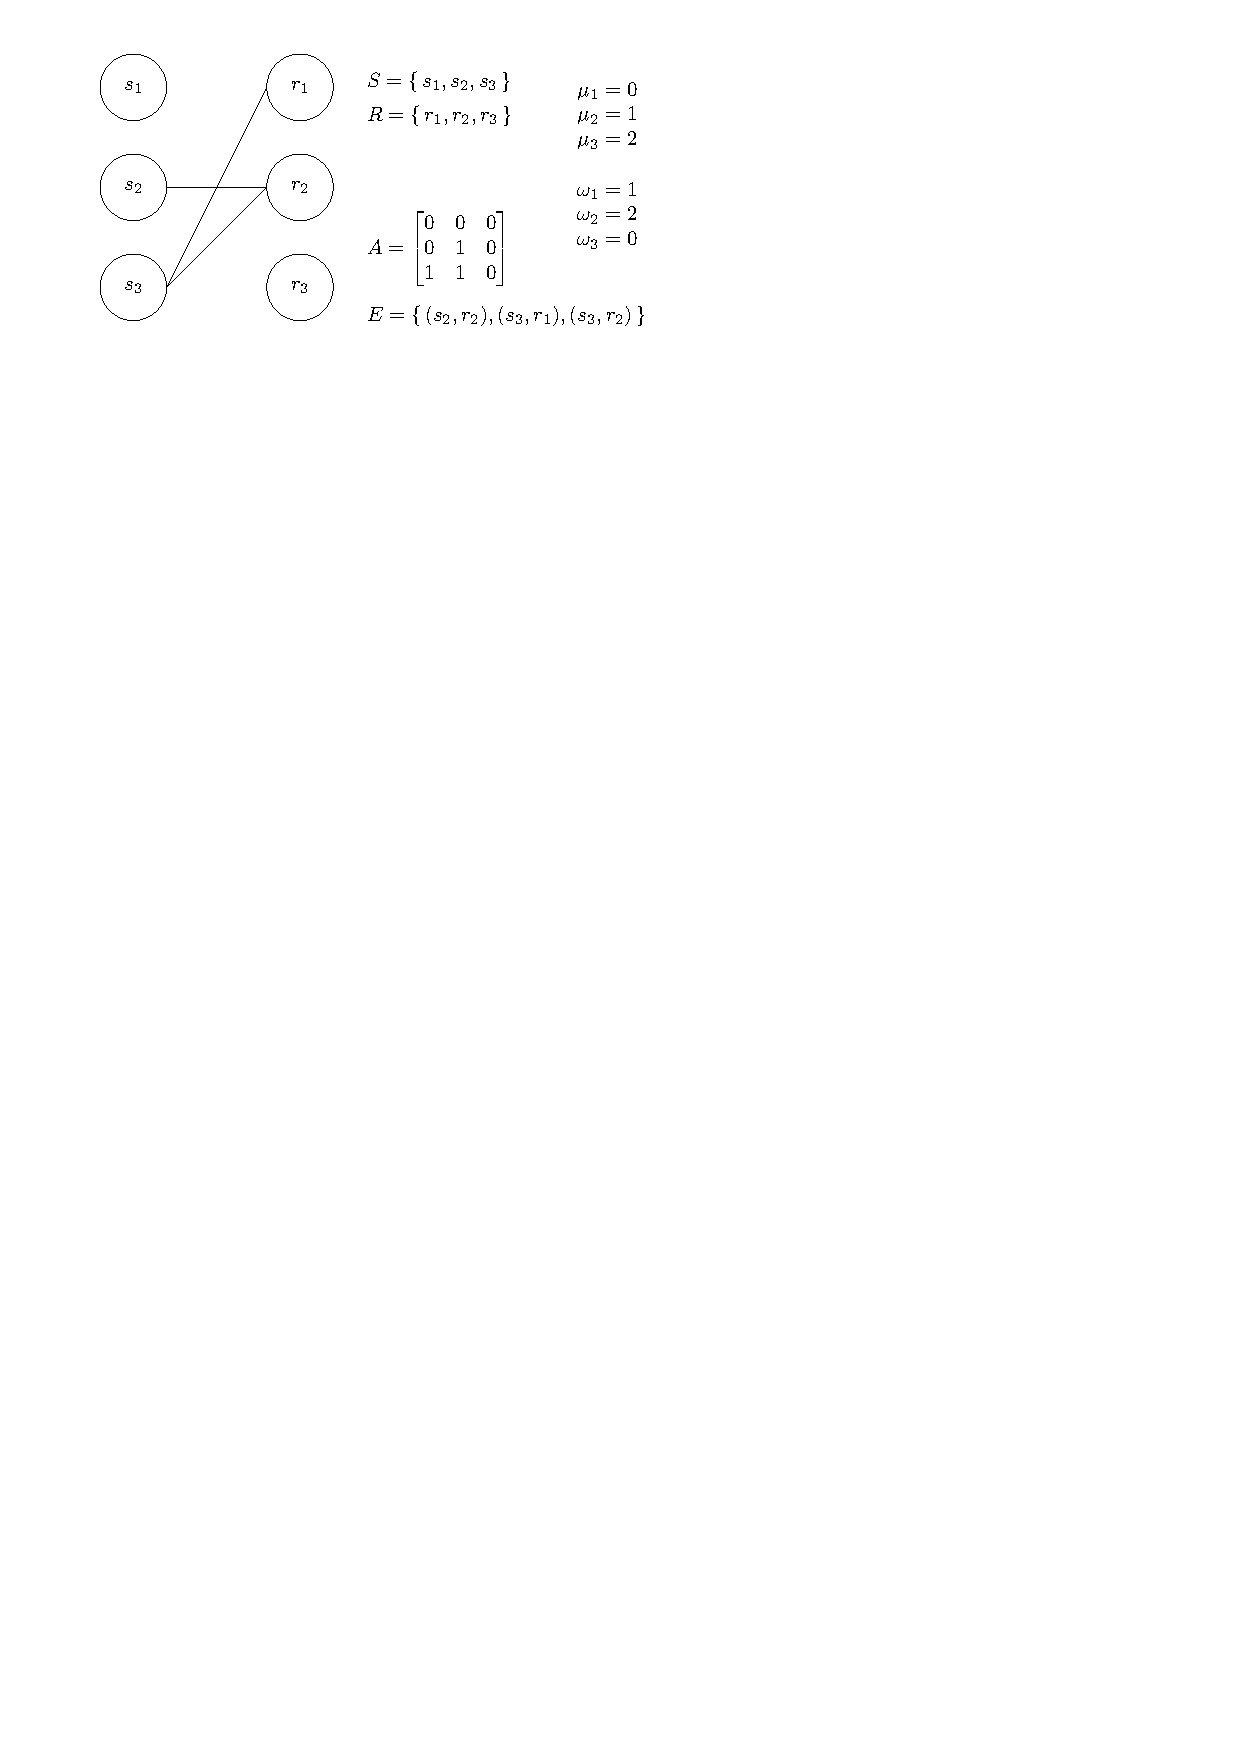
\includegraphics[width=\textwidth]{graph_example_base}
  \caption{%
    A bipartite graph with the corresponding adjacency matrix $A$, set of edges $E$ and vertex degrees $\mu$ and $\omega$ for each vertex.
  }
  \label{fig:graph-example-base}
\end{figure}

\subsection{Information theory}
\label{sec:introduction_model_info-theory}

Information theory measures are used to compute the cost function of the optimization process.
Here we go through a short overview of information theory formulas.

The general formula for the entropy of a set $X$ is
\begin{equation}
  \label{eq:definition-entropy-generic}
  H(X) = \sum_{x \in X} p(x) \log p(x)
\end{equation}
where $p(x)$ is the probability associated with the element $x$.
The general formula for the joint entropy of two sets $X$ and $Y$ is defined as
\begin{equation}
  \label{eq:definition-joint-entropy-generic}
  H(X,Y) = \sum_{x \in X} \sum_{y \in Y} p(x,y) \log p(x,y)
\end{equation}
where $p(x,y)$ is the joint probability of the elements $x$ and $y$.

Any other information theoretic measures concerning two sets can be obtained from $H(X)$, $H(Y)$ and $H(X,Y)$.
Mutual information
\begin{equation*}
  I(X,Y) = H(X) + H(Y) - H(X,Y),
\end{equation*}
and conditional entropies
\begin{equation*}
  H(X|Y) = H(X,Y) - H(X)
\end{equation*}
and
\begin{equation*}
  H(Y|X) = H(X,Y) - H(Y).
\end{equation*}
The diagram on Figure \ref{fig:relationships-entropies} shows these relationships in a more visual way.

\begin{figure}
  \centering
  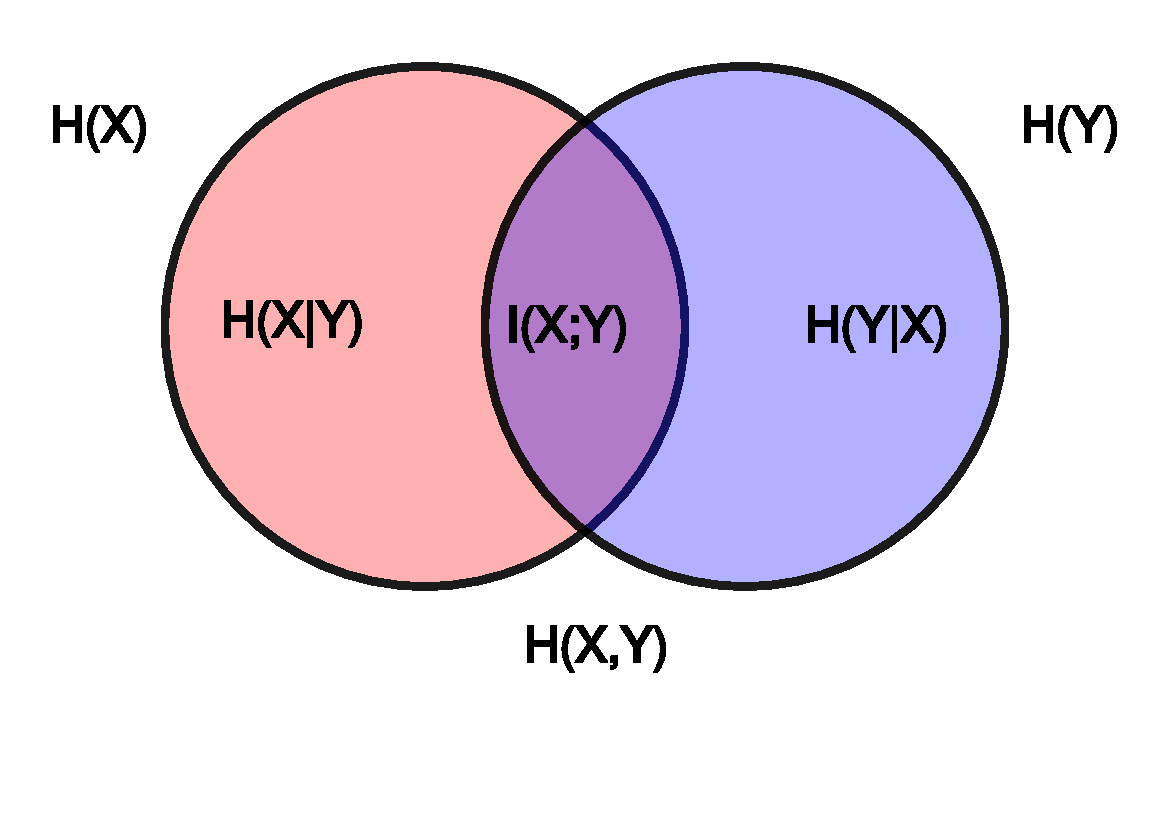
\includegraphics[width=\textwidth]{relationships_entropies}
  \caption{
    This diagram illustrates the relationships between information theoretic measures for two sets $X$ and $Y$.
    The area occupied by both left and right circle is the joint entropy $H(X,Y)$.
    The circle on the left (both the red and the violet areas) represents the marginal entropy $H(S)$ while the circle on the right (both blue and violet areas) represents the marginal entropy $H(Y)$.
    The red area is the conditional entropy $H(X|Y)$ while the blue area represents the conditional entropy $H(Y|X)$.
    The violet area represents the mutual information $I(X,Y)$.
  }
  \label{fig:relationships-entropies}
\end{figure}

Based on Equation \ref{eq:definition-entropy-generic}, we define the entropies of words and meanings, $H(S)$ and $H(R)$ respectively, as
\begin{equation}
  \label{eq:definition-HS}
  H(S) = \sum_{i=1}^n p(s_i) \log p(s_i)
\end{equation}
and
\begin{equation}
  \label{eq:definition-HR}
  H(R) = \sum_{j=1}^m p(r_j) \log p(r_j).
\end{equation}
We also define the joint entropy of words and meanings, from Equation \ref{eq:definition-joint-entropy-generic}, as
\begin{equation}
  \label{eq:definition-HSR}
  H(S,R) = \sum_{i=1}^n \sum_{j=1}^m p(s_i, r_j) \log p(s_i, r_j).
\end{equation}

\subsection{The $\phi$ parameter}
\label{sec:introduction_model_phi}

\redtxt{(we're making more general versions of previous model which now depend
  on more stuff but can be brought back to previous models by setting phi to
  0)}

The $\phi$ parameter, which has already appeared up to this point, is used to generalize the older versions of the two main models studied.

In \cite{Ferrer2005a} and \cite{Ferrer2003a} these two models were introduced.
Later, the $\phi$ parameter is added to generalize the model and hopefully be able to predict more linguistic laws \cite{Ferrer2018a}.

As is presented in the following sections, when $\phi=0$, the older models are retrieved from the newer ones.

\subsection{The \firstmodel{}}
\label{sec:introduction_model_first-model}

In this model, the joint probability of a word $s_i$ and a meaning $r_j$ is proportional to the product of their degrees to the $\phi$ power.
When $\phi=0$, the joint probability depends only on whether there is a connection between the word and the meaning.
Mathematically,
\begin{equation*}
  \label{eq:psirj-proportional-mui-wj}
  p(s_i, r_j) \propto a_{i,j} (\mu_i \omega_j)^\phi.
\end{equation*}
When $\phi=0$ we recover a previous simpler model \cite{Ferrer2005a}.

The actual joint probability is derived from Equation \ref{eq:psirj-proportional-mui-wj}, and from it the marginal probabilities of words and meanings are also derived.
Ultimately this leads to the information theoretic equations seen in Section \ref{sec:introduction_model_info-theory}.

\subsection{The \secondmodel{}}
\label{sec:introduction_model_second-model}

This model was introduced in \cite{Ferrer2003a} with meaning probabilities being constant and disconnected meanings being disallowed.
Here we present a generalization of the previous model.
In this model, the probability of a meaning $r_j$ is given \emph{a priori} as $\pi(r_j)$.
It is possible for a meaning to be disconnected from any words, in which case $p(r_j) = 0$.
In \cite{Ferrer2003a} disconnected meanings were disallowed and $\pi(r_j) = \frac{1}{m}$.
Additionally, $\phi=0$ in Equation \ref{eq:prop-cond-prob_second-model}.
Here $\pi(r_j)$ can follow any probability distribution and disconnected meanings are allowed.
Zero values of $\pi(r_j)$ are disallowed, however, as meanings that could never occur are not the target of communication.

We then define $p(r_j)$ as
\begin{equation}
  \label{eq:prj-proportional-pirj}
  p(r_j) \propto (1 - \delta_{\omega_j,0}) \pi(r_j)
\end{equation}
where $\delta_{a,b}$ is the Kronecker delta,
\begin{equation*}
  \delta_{a,b} = \begin{cases}
    0 & \text{if}~a \neq b \\
    1 & \text{if}~a = b.
  \end{cases}
\end{equation*}
The word probability is then defined as the conditional probability of choosing a word given that a meaning has been chosen,
\begin{equation}
  \label{eq:prop-cond-prob_second-model}
  p(s_i | r_j) \propto a_{i,j} \mu_i^\phi.
\end{equation}

With the marginal meaning probability and the conditional probability of a word given a meaning, the joint probability and marginal word probability can be calculated.
From this the information theoretic equations are be obtained.

\subsection{Optimization}
\label{sec:introduction_model_optimization}

As seen in previous sections and will be seen in Section \ref{sec:introduction_hypothesis}, our hypothesis is that the empirical laws observed in human language are the result of minimizing the effort of speaker and hearer.

This effort is defined in terms of information theoretic measures.
We choose two competing forces.
$H(S)$, the entropy of the words, and $I(S,R)$, the mutual information between words and meanings.
It is the goal of any communications system to maximize $I(S,R)$. The smaller $I(S,R)$, the greater the effort for the hearer.
The higher the entropy of words, however, they harder they are to access.
When $H(S)=0$, only a single word has probability 1 while all others are 0, meaning that knowing which word to choose is trivial, while $H(S)$ is maximum when all words have equal probability, giving no indication of which should be chosen.

We define $\Omega(\lambda)$ as the cost function we aim to minimize,
\begin{equation}
  \label{eq:definition-Omega}
  \Omega(\lambda) = -\lambda I(S,R) + (1 - \lambda) H(S)
\end{equation}
where $0 \leq \lambda \leq 1$ is used to indicate the weight given to each of the two forces.
When $\lambda=0$, the minimization of $H(S)$ is completely favored while when $\lambda=1$ the maximization of $I(S,R)$ is.
When $\lambda=1/2$, they are equally favored.

The optimization process follows a Markov chain Monte Carlo method at zero temperature.
It consists of making mutations to $A$, chancing $a_{i,j}$ from 1 to 0 or from 0 to 1.
If a set of mutations results in a decrease of $\Omega$, they are kept.
Otherwise they are undone and another set is attempted.

\subsection{Dynamic and static equations}
\label{sec:introduction_model_dynamic-static}

As is seen later on, in Chapter \ref{cha:model}, two sets of equations are derived for the information theoretic equations necessary to calculate $\Omega$ (Equation \ref{eq:definition-Omega}).

A set of static equations recalculate everything from scratch.
The set of dynamic equations calculate the changes done only after a mutation to $A$ takes place.

As seen in Section \ref{sec:introduction_background_similar} this dynamic recalculation can be more efficient.
In the case of this thesis, small changes are continuously done to the graph, making several mutations to $A$ then reevaluating $\Omega$.
Dynamically accounting for the differences brought about for these changes is much more efficient than recalculating every single measure each time.

Dynamic calculation, however, brings its own set of problems, such as the increase in mathematical complexity and the introduction of greater floating point error.
Section \ref{sec:introduction_challenges_dynamic} goes over this in more detail while Section \ref{sec:methods_model-implementation} covers the measures taken in order to deal with these problems.

\section{Goals}
\label{sec:introduction_goals}

With the model introduced, more specific goals are stated. See also the overall goals in section \ref{sec:introduction_general-goals}.

\begin{itemize}
\item
  To create an open source tool implementing the general models.
  \begin{itemize}
  \item
    This tool should be both powerful and flexible, allowing to replicate previous results for the case $\phi=0$.
  \item
    It should also be efficient and fast enough that results with relatively large graphs can be obtained in a reasonable time. This means using dynamic equations.
  \item
    It should be relatively easy to use such that anyone who wishes to test these models by themselves can do it.
  \end{itemize}
\item
  Find out whether local minima exist.
  It is not clear whether there exists local minima for the case $\phi \neq 0$.
  The previous models where $\phi = 0$ have been analyzed mathematically \cite{Salge2015} \cite{Prokopenko2010}.
  The case $\phi \neq 0$ is more complex and would be very hard to analyze mathematically to this level.
  It is possible that the optimization stops at a point where the function could still be minimized further but it is hard to find the set of mutations that minimize it.
  Or it could be that the function does reach a local minima.
\end{itemize}

\section{Hypothesis}
\label{sec:introduction_hypothesis}

Several hypothesis are stated here.

As seen in section \ref{sec:introduction_background} and in \cite{Ferrer2018a}, there is a relationship between the exponents of the Zipf's word-frequency and meaning-frequency laws.
See Equation \ref{eq:relation-exponents}.
The main hypothesis of the thesis is that linguistic laws appear due to an optimization process.
It is under this assumption that the entire model works and the results are obtained.
In the model we also neglect any effects of social interaction, which are the basis of other approaches to investigating human language such as the naming game \cite{Baronchelli2006}.
Another hypothesis is that the optimization process does not necessarily arrive at a local minimum.

\section{Challenges}
\label{sec:introduction_challenges}

The main challenges presented by this thesis are outlined here.
They are divided into three categories: challenges relating to quantitative linguistics in Section \ref{sec:introduction_challenges_quant-lin}, computational challenges in Section \ref{sec:introduction_challenges_computational} and the challenges brought by the use of a dynamic calculation technique, in section \ref{sec:introduction_challenges_dynamic}.

\subsection{Quantitative linguistics}
\label{sec:introduction_challenges_quant-lin}

The challenges relating to quantitative linguistics come from the fact that current models already can make some predictions.
Can these new models predict anything new? Can they still make the predictions that the old models already could?
Specifically, the $\phi=0$ models presented in \cite{Ferrer2005a} and \cite{Ferrer2003a} already showed the appearance of Zipf's law of word frequencies.
Can the new models with $\phi \neq 1$ (and more specifically $\phi=1$) make any new predictions such as the law of meaning frequency, or the one relating word ages and frequencies?
Can they still predict Zipf's law?

\subsection{Computational}
\label{sec:introduction_challenges_computational}

The computational challenges relate to the implementation of the model.

Verification is a very important step.
The mathematics are complex, specially in the dynamic case, and a single mistake can invalidate all the results.
Therefore, the implementation must be verified thoroughly and completely.

The stop condition of the optimization process is also difficult to properly implement.
The algorithm should stop once it can be reasonably sure that a minimum has been reached.
However, due to the size search space, it is unfeasible to check every possible set of mutations.

An important challenge is recalculating $\Omega$ efficiently enough that results with relatively big $n$ and $m$ can be executed in a reasonable time.
The calculation of $\Omega$ directly influences the runtime of the program.
In order to speed it up, dynamic calculations are used.
Dynamic calculation, however, presents its own set of challenges.

\subsection{Dynamic calculation}
\label{sec:introduction_challenges_dynamic}

Dynamic calculation is much more mathematically complex than static calculation.
This complexity makes the likelihood of a bug being introduced much more likely.
Therefore the verification process must be even more thorough.

In addition to complexity, dynamic calculation implies many addition and subtraction operations.
These operations introduce greater floating point error than others (such as multiplication and division).
If the floating point error accumulates, it can change the result into a different one from the static method.
Dynamic and static approaches should lead to identical results.

\section{Outline of the thesis}
\label{sec:introduction_outline}

The rest of the thesis is organized as follows:

Chapter \ref{cha:model} gives more detail of the models, and all the mathematical detail concerning the models (although long derivations or simple proofs that are otherwise unrelated are left for Appendix \ref{cha:app_formulae}).
It is during this chapter that all the mathematics that are eventually implemented into the open source tool are showcased.
The computational aspects are also seen here, showing the computational complexity of implementing these formulas.
This chapter starts from the initial concepts seen in Section \ref{sec:introduction_model}.

Chapter \ref{cha:methods} goes into the implementation of the model.
It includes full descriptions of various implementation details, of the optimization algorithm, the decisions regarding parallelization of the code and the approach to verification.
It also covers some challenges unique to the implementation of the model and how they were resolved.

Chapter \ref{cha:results} introduces the results obtained from the open source tool.
It includes the figures from the previous models \cite{Ferrer2005a} and \cite{Ferrer2003a} implemented with $\phi=0$.
It also includes new data obtained by setting $\phi=1$.

Finally, Chapter \ref{cha:discussion} discusses the obtained results and their relation to certain linguistic laws that have been seen in this introduction.
Future work is also discussed in this chapter, including alternative optimization methods.

%%% Local Variables:
%%% mode: latex
%%% TeX-master: "tfm"
%%% End:
